\documentclass[a4paper,12pt]{article}

\usepackage{babel}
\usepackage{graphicx}
\usepackage{float}
\usepackage{enumitem} 
\usepackage{hyperref}
\usepackage{caption}
\usepackage{url}


\begin{document}

\title{Comparative analysis of connected component for Bengali Character recognition.}

\author{
  Pritilata Biswas\\
  \texttt{1103017}
  \and
  Sumaia Afrin Prity\\
  \texttt{1103057}
  \and
  Parvez Abedin Siddique\\
  \texttt{1103094}\\
  \texttt{Section A}\\
  \texttt{Level 4, Term 2}\\
  \texttt{Department of Computer Science and Engineering}\\
  \texttt{BAIUST}
}

\date{\today}

\maketitle

\section{Topic Characteristics}

\paragraph*{Segmentation of Bangla handwritten text is the pre-process of handwritten text. The bengali script is also used for representing other language like Meithei and Bishnupriya Manipuri, and there is time when it used to write Sanskrit within Bengal \hyperlink{1}{[1]}. Most of the Bengali characters are topologically connected \hyperlink{2}{[2]}. They can be easily classified using this connectedness property. This classifying or segmentation of Bengali character is the most challenging task in making a Bengali Optical Character Recognition (OCR). In Bengali there is a combination of basic, modified and compound characters. The combination of characters can be more than 300. Here, Bengali character segmentation is the most challenging task. So, we need some robust techniques that can classify these compound characters.} 

\paragraph*{We know Bengali script characters are connected with a Matra line, so the characters can be easily recognized by the connected component analysis \hyperlink{2}{[2]}. In this paper our main contribution is to improvise the method of analyzing connected component using some common image processing operations. }

\paragraph*{In this 21st century of digital generation, OCR is one the most important technique to interface between human and machines. OCR of printed text has already achieved a huge success. ABBYY is one of the major examples of most fine reader that is commercially available \hyperlink{3}{[3]}. A little works has been done on Bengali Handwritten character recognition \hyperlink{9}{[9]}, \hyperlink{10}{[10]}, \hyperlink{11}{[11]}, \hyperlink{12}{[12]}. Now, an efficient Bangla OCR system is important to be developed. Many researchers have already developed many methods of segmentation of Bengali script. }

\paragraph*{Chaudhuri et al \hyperlink{9}{[9]} first proposed an OCR system using HPP and VPP and headline removal technique they segmented the documents into lines, words, and characters. Mahmud et al \hyperlink{10}{[10]} first proposed an that supports multi font characters. Mahmud et al \hyperlink{11}{[11]} used Depth First Search (DFS) algorithm for overlapped character segmentation. Hasan et al \hyperlink{12}{[12]} proposed a hamming network for Segmentation. All of these method, they divide the words into three regions (matra line, upper zone, lower zone). For dividing them into regions one of the best approaches is to detect the Matra line and remove them. But removing them incurs some major problems in most of the characters as they are incomplete without their Matra line. So, in this paper we proposed a method that may counter this problem.}

\section{Objective}

\begin{itemize}

\item To enhance Bengali connected component analysis
\item To improvise Profile Projection with Opening, Closing operations
\item To implement Opening, Closing operations, Profile Projection with Erosion, Dilation operations are needed.
\item Comparative analysis between existing and proposed method.

\end{itemize}

\section{Working Hypothesis}

\paragraph*{A typical OCR system consists of preprocessing, segmentation, recognition and post-processing parts. In this paper we mainly focused on the segmentation process which is the back bone of the recognition phase.}

\paragraph*{At first the input image will be converted into grayscale image using grayscale filter and using bilateral filter we will remove the noise in the input image. Then using bit plane slicing the input image will be binarized and will be converted into two-tone image. Some input image may be skewed by a few degrees. For skew correction we will use the skew angle technique \hyperlink{4}{[4]}.}

\paragraph*{In Bengali script, lines are almost of the same height. There is a horizontal gap between two lines. We will detect those gapes by horizontal projection profile (HPP). Vertical projection profile (VPP) will be used in word segmentation from extracted lines. In this process the number of black pixels in each column will be calculated. In vertical scan if no black pixel found then it will be considered as the gap between words.}

\paragraph*{Bengali words are connected through Matra line. By removing them, characters get topologically disconnected. Then using the connected component method, individual components of a word can be separated. Now we will apply erosion and dilation to remove the problems that will occur from the removal of Matra line. Finally, we will analyze the connected component (each character) how close they are.}

\clearpage

\section{Methodology}

\begin{figure}[h!]
\centering
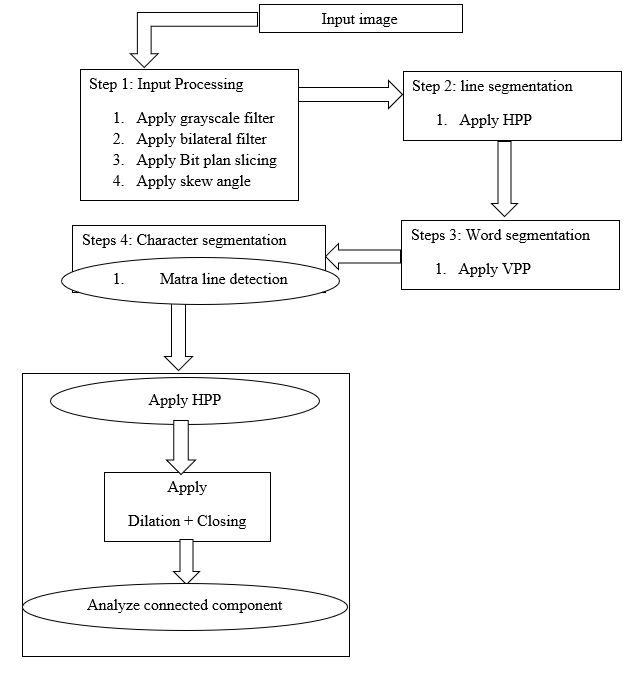
\includegraphics[width=1.2\textwidth]{fig_1.png}
\caption{The proposed methodology}
\end{figure}

\section{References}

\begin{enumerate}

\item \hypertarget{1}{\url{https://en.wikipedia.org/wiki/Bengali_alphabet}}
\item \hypertarget{2}{T. Zahan, M.R. Selim, M.S. Rahman, M.Z. Iqbal, (2018). \textit{“Connected Component Analysis Based Two Zone Approach for Bangla Character Segmentation.”} 1-4. 10.1109/ICBSLP.2018.8554684.}
\item \hypertarget{3}{\url{https://www.abbyy.com/ . Last accessed 07 Dec 2016}}
\item \hypertarget{4}{M. A. Obaida, T. K. Roy, M. A. Horaira and M. J. Hossain, \textit{“Skew Correction Function of OCR: Stroke-Whitespace based Algorithmic Approach,”} International Journal of Computer Applications 28(8):7-12, August 2011}
\item \hypertarget{5}{S. S. Goswami, \textit{“Identification of Matra Region and Overlapping Characters for OCR of Printed Bengali Scripts,”} Intelligent Computing and Information Science, Volume 135 of the series Communications in Computer and Information Science, 2011, pp. 606-612}
\item \hypertarget{6}{\url{https://docs.opencv.org/2.4/doc/tutorials/imgproc/erosion_dilatation/erosion_dilatation.html}}
\item \hypertarget{7}{\url{https://homepages.inf.ed.ac.uk/rbf/HIPR2/open.htm}}
\item \hypertarget{8}{\url{https://homepages.inf.ed.ac.uk/rbf/HIPR2/close.htm}}
\item \hypertarget{9}{B. B. Chaudhuri and U. Pal, “A Complete Printed Bangla OCR System,” Pattern Recognition, Vol. 31, No. 5, pp. 531—549, 1998.}
\item \hypertarget{10}{J. U. Mahmud, M. F. Raihan and C. M. Rahman, \textit{“A complete OCR system for continuous Bengali characters,”} In: Proceedings of the TENCON, 1372–1376, 2003.}
\item \hypertarget{11}{S. M. M. Mahmud, N. Shahrier, A.S.M D. Hossain, M. T. M. Chowdhury, and M.A. Sattar, \textit{“An Efficient Segmentation Scheme for the Recognition of Printed Bangla characters,”} Proceedings of ICCIT, pp 283-286, 2003.}
\item \hypertarget{12}{M. A. M. Hasan, M. A. Alim, and M. W. Islam \textit{“A New Approach to Bangla Text Extraction and Recognition from Textual Image”}, Proceedings of ICCIT, 2005.}

\end{enumerate}


\end{document}